% MBDyn (C) is a multibody analysis code.
% http://www.mbdyn.org
%
% Copyright (C) 1996-2023
%
% Pierangelo Masarati  <pierangelo.masarati@polimi.it>
%
% Dipartimento di Ingegneria Aerospaziale - Politecnico di Milano
% via La Masa, 34 - 20156 Milano, Italy
% http://www.aero.polimi.it
%
% Changing this copyright notice is forbidden.
%
% This program is free software; you can redistribute it and/or modify
% it under the terms of the GNU General Public License as published by
% the Free Software Foundation (version 2 of the License).
%
%
% This program is distributed in the hope that it will be useful,
% but WITHOUT ANY WARRANTY; without even the implied warranty of
% MERCHANTABILITY or FITNESS FOR A PARTICULAR PURPOSE.  See the
% GNU General Public License for more details.
%
% You should have received a copy of the GNU General Public License
% along with this program; if not, write to the Free Software
% Foundation, Inc., 59 Temple Place, Suite 330, Boston, MA  02111-1307  USA

\section{Surface Loads}
\label{sec:EL:SURFLOAD}

\emph{Author: Reinhard Resch}
\subsection{Pressure Loads}
Pressure loads are intended mainly to apply prescribed pressure boundary conditions at the surface of solid elements.
However, they could be used also for shell and membrane elements. The value of the pressure can be imposed
by means of a set of drive callers, or by means of a set of abstract nodes. By convention, pressure loads are always applied
in the opposite direction of the surface normal vector. So, it is important, that the surfaces are oriented properly
when creating the mesh (e.g. use \emph{ReorientMesh} in \htmladdnormallink{\texttt{Gmsh}}{https://gmsh.info/}).
See also table~\ref{sec:EL:SURFLOAD:elemtypes} for a list of supported elements.
\begin{Verbatim}[commandchars=\\\{\}]
  \bnt{elem_type} ::= \{ \kw{pressureq4} | \kw{pressureq8} | \kw{pressureq8r} | \kw{pressuret6} \}

    \bnt{normal_arglist} ::=
        \bnt{struct_node_data} , \bnt{pressure_load_data} ;

     \bnt{struct_node_data} :: =
        (\ty{StructDispNode}) \bnt{struct_node_1_label} ,
        (\ty{StructDispNode}) \bnt{struct_node_2_label} ,
        ... ,
        (\ty{StructDispNode}) \bnt{struct_node_N_label}

     \bnt{pressure_load_data} :: =
        \{ \kw{from drives} , \bnt{press_drive_data} |
           \kw{from nodes}  , \bnt{press_node_data} \}

      \bnt{pressure_drive_data} :: =
        (\hty{DriveCaller}) \bnt{press_drive_1} ,
        (\hty{DriveCaller}) \bnt{press_drive_2} ,
        ... ,
        (\hty{DriveCaller}) \bnt{press_drive_N}

      \bnt{pressure_node_data} :: =
        (\ty{AbstractNode}) \bnt{press_node_1} ,
        (\ty{AbstractNode}) \bnt{press_node_2} ,
        ... ,
        (\ty{AbstractNode}) \bnt{press_node_N}

\end{Verbatim}

\subsubsection{Example:}
\begin{verbatim}
       drive caller: 1, string, "1.5 * Time";
       drive caller: 2, string, "2.5 * Time";
       drive caller: 3, string, "3.5 * Time";
       drive caller: 4, string, "4.5 * Time";

       pressureq4: 100, 1, 2, 3, 4, from nodes, 10, 11, 12, 13;

       pressureq4: 101, 5, 6, 7, 8, from drives,
                    reference, 1,
                    reference, 2,
                    reference, 3,
                    reference, 4;
\end{verbatim}

\subsection{Surface Traction's}
Surface traction's are similar to pressure loads but they do not necessarily act perpendicular to the surface.
So, they can be used to impose a prescribed shear stress at the surface of a solid body.
Actually there are absolute and relative surface traction's. Absolute surface traction's are applied with respect
to the global reference frame and do not change their direction and magnitude if the surface is moved
or deformed during the simulation. In contradiction to that, relative surface traction's are also applied with respect
to the global reference frame, but their direction and magnitude is changed similar to pressure loads, if the surface is deformed or moved.
See also table~\ref{sec:EL:SURFLOAD:elemtypes} for a list of supported elements.
\begin{Verbatim}[commandchars=\\\{\}]
  \bnt{elem_type} ::= \{ \kw{tractionq4} | \kw{tractionq8} | \kw{tractionq8r} | \kw{tractiont6} \}

    \bnt{normal_arglist} ::=
        [ \kw{absolute} , ] \bnt{struct_node_data} , \kw{from drives} , \bnt{traction_load_data}
        [ , \kw{orientation}, \bnt{traction_orient_data} ] ;

     \bnt{struct_node_data} :: =
        (\ty{StructDispNode}) \bnt{struct_node_1_label} ,
        (\ty{StructDispNode}) \bnt{struct_node_2_label} ,
        ... ,
        (\ty{StructDispNode}) \bnt{struct_node_N_label}

     \bnt{traction_load_data} :: =
        (\htybty{TplDriveCaller}{Vec3}) \bnt{traction_stress_1} ,
        (\htybty{TplDriveCaller}{Vec3}) \bnt{traction_stress_2} ,
        ... ,
        (\htybty{TplDriveCaller}{Vec3}) \bnt{traction_stress_N}

     \bnt{traction_orient_data} :: =
        (\hty{OrientationMatrix}) \bnt{orientation_matrix_1} ,
        (\hty{OrientationMatrix}) \bnt{orientation_matrix_2} ,
        ... ,
        (\hty{OrientationMatrix}) \bnt{orientation_matrix_M}
\end{Verbatim}

\subsubsection{Example:}
\begin{verbatim}
       reference: 10,
                position, reference, global, null,
                orientation, reference, global, 1, 0., 1., 0.,
                                                2, 1., 0., 0.,
                velocity, reference, global, null,
                angular velocity, reference, global, null;

       ...

       template drive caller: 1, 3, component,
                string, "1.5 * Time",
                string, "2.5 * Time",
                string, "3.5 * Time";

       ...

       template drive caller: 4, 3, component,
                string, "4.5 * Time",
                string, "5.5 * Time",
                string, "6.5 * Time";

       tractionq4: 100, 1, 2, 3, 4, from drives,
                    reference, 1,
                    reference, 2,
                    reference, 3,
                    reference, 4,
                    orientation,
                       reference, 10, eye,
                       reference, 20, eye,
                       reference, 30, eye,
                       reference, 40, eye;
\end{verbatim}

\begin{table}[h!tp]
\begin{tabular}[t]{|c|c|c|c|c|c|c|}
  \hline
  element type pressure & element type traction & nodes & node order & integration points & order & references \tabularnewline
  \hline
  \kw{pressureq4} & \kw{tractionq4} & 4 & \ref{fig:EL:SURFLOAD:QUADRANGLE4} & 4 & 1 & \cite{BATHE2016} \tabularnewline
  \hline
  \kw{pressureq8} & \kw{tractionq8} & 8 & \ref{fig:EL:SURFLOAD:QUADRANGLE8} & 9 & 2 & \cite{BATHE2016} \tabularnewline
  \hline
  \kw{pressureq8r} & \kw{tractionq8r} & 8 & \ref{fig:EL:SURFLOAD:QUADRANGLE8R} & 9 & 2 & \cite{DHONDT2004} \tabularnewline
  \hline
  \kw{pressuret6} & \kw{tractiont6} & 6 & \ref{fig:EL:SURFLOAD:TRIANGLE6H} & 7 & 2 & \cite{CODEASTERR30301} \tabularnewline
  \hline
\end{tabular}
  \caption{Finite Element Types for surface loads}
  \label{sec:EL:SURFLOAD:elemtypes}
\end{table}

\begin{figure}[htb]
\centering
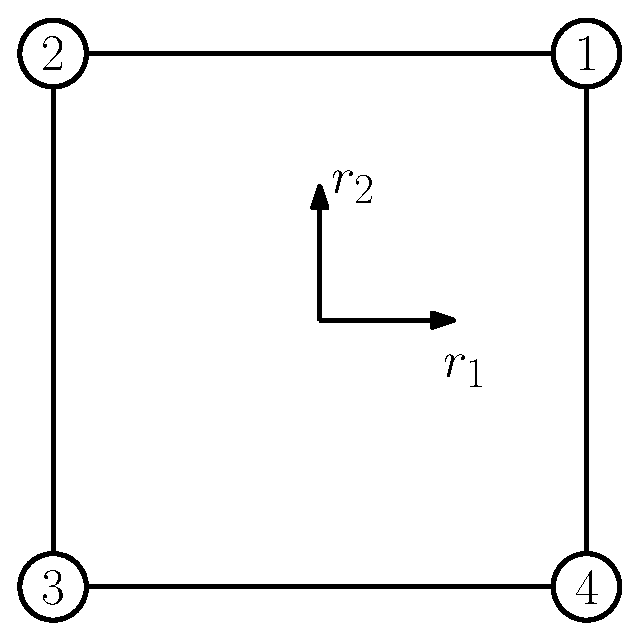
\includegraphics[width=.25\textwidth]{quadrangle4}
\caption{Node order: \kw{pressureq4}, \kw{tractionq4}}
\label{fig:EL:SURFLOAD:QUADRANGLE4}
\end{figure}

\begin{figure}[htb]
\centering
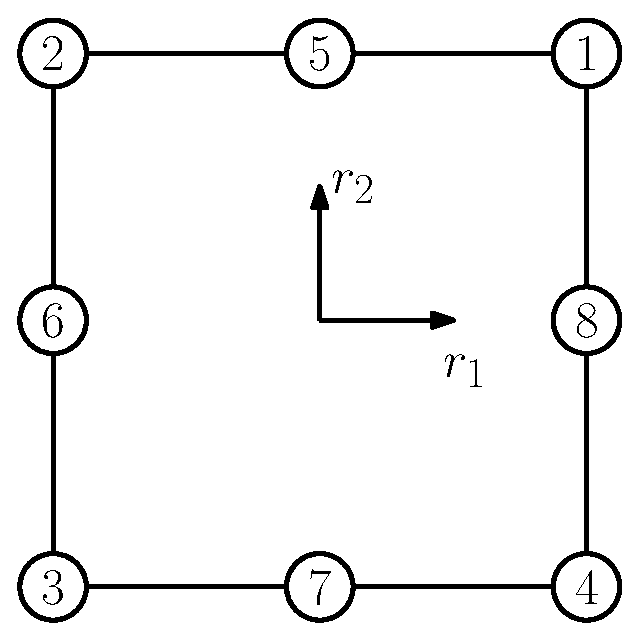
\includegraphics[width=.25\textwidth]{quadrangle8}
\caption{Node order: \kw{pressureq8}, \kw{tractionq8}}
\label{fig:EL:SURFLOAD:QUADRANGLE8}
\end{figure}

\begin{figure}[htb]
\centering
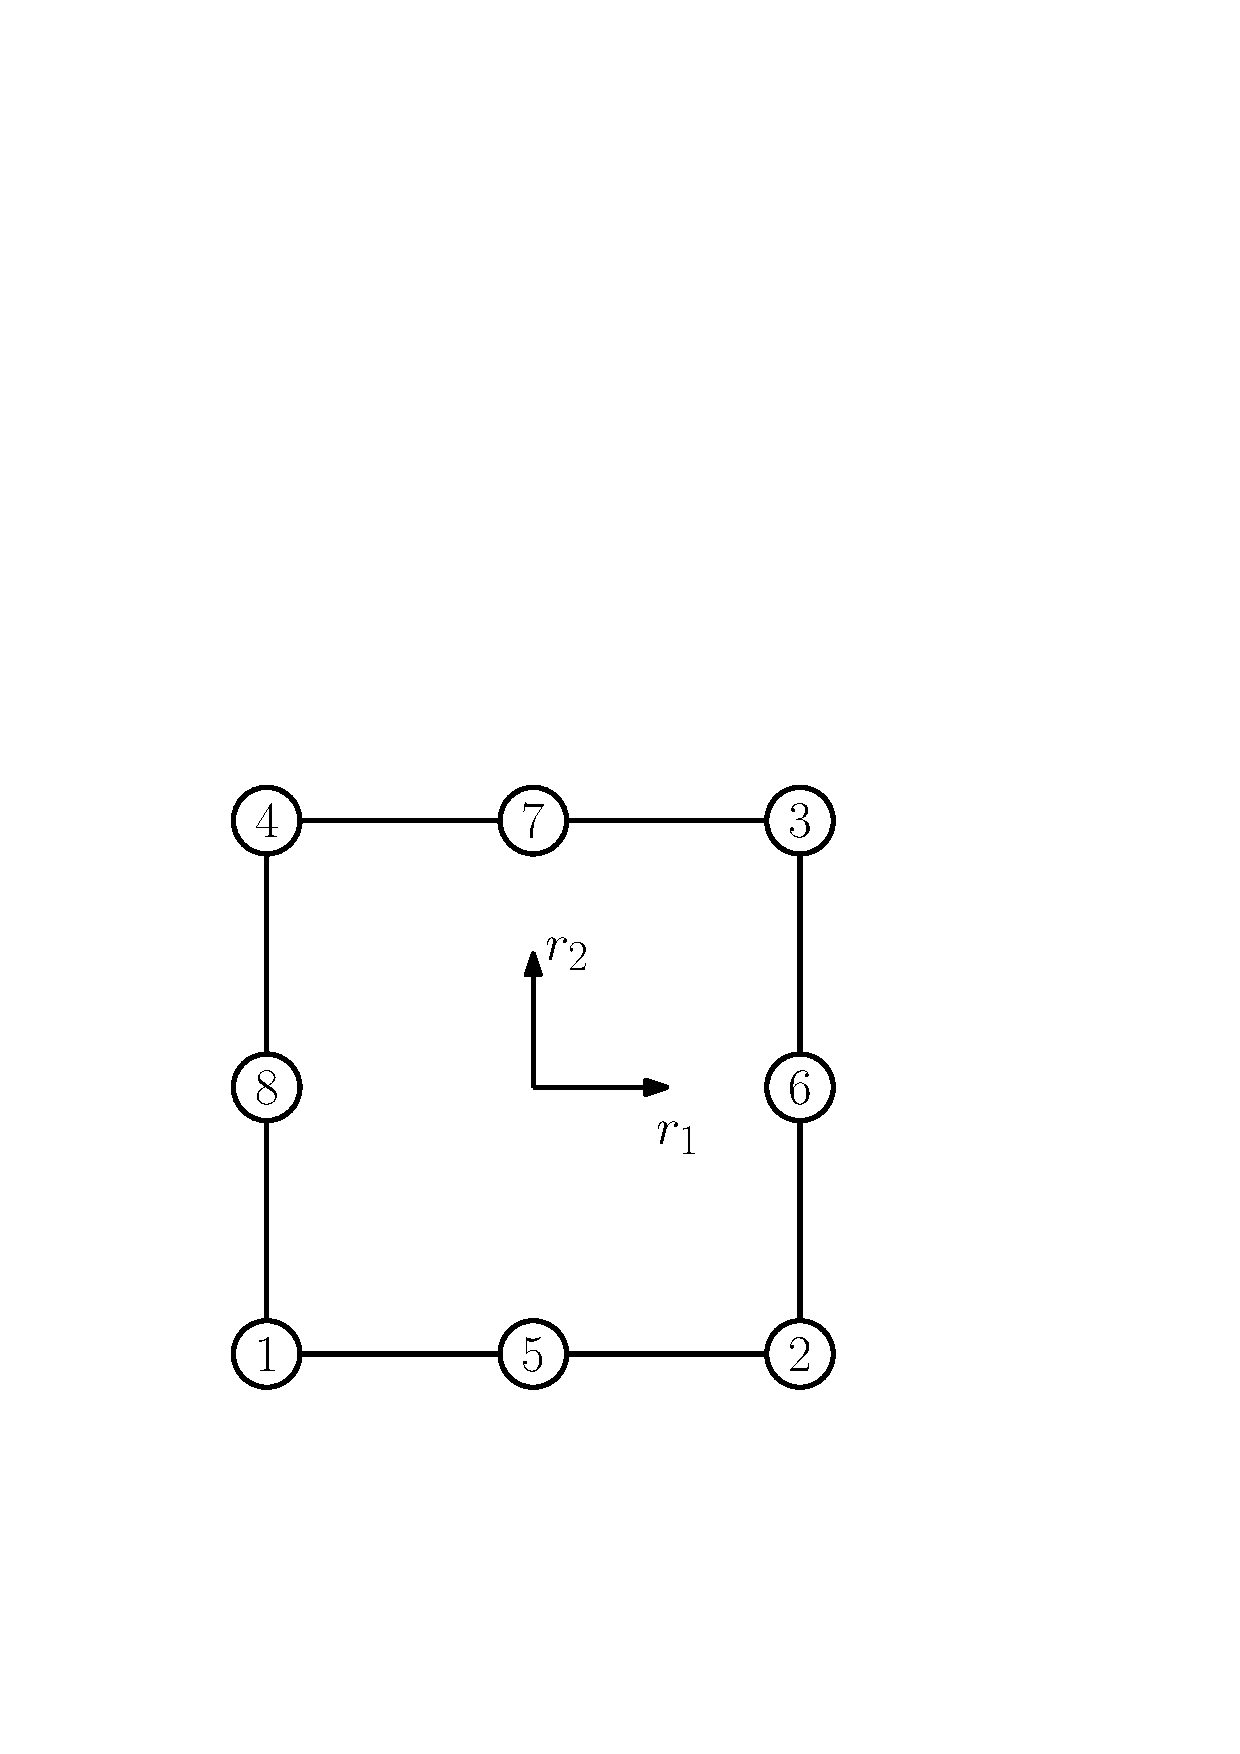
\includegraphics[width=.25\textwidth]{quadrangle8r}
\caption{Node order: \kw{pressureq8r}, \kw{tractionq8r}}
\label{fig:EL:SURFLOAD:QUADRANGLE8R}
\end{figure}

\begin{figure}[htb]
\centering
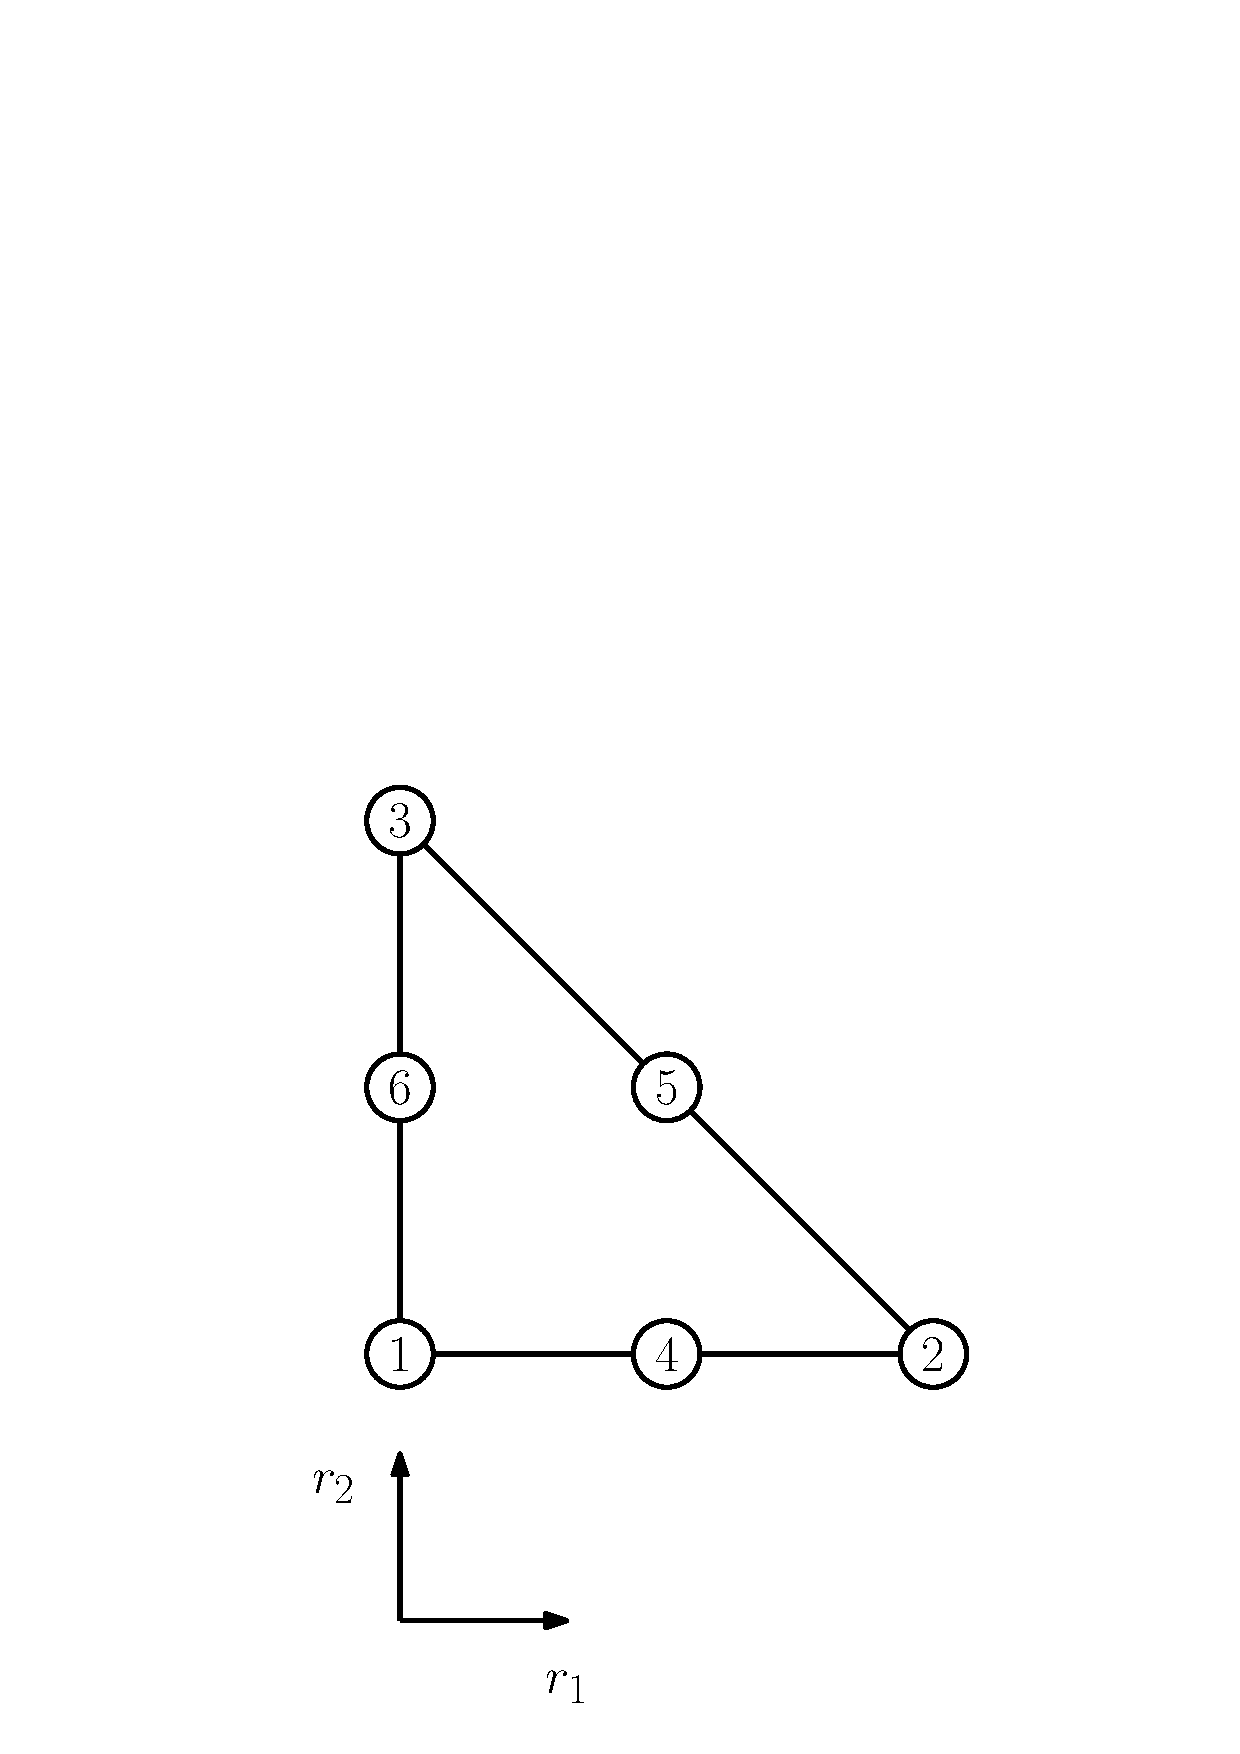
\includegraphics[width=.25\textwidth]{triangle6h}
\caption{Node order: \kw{pressuret6}, \kw{tractiont6}}
\label{fig:EL:SURFLOAD:TRIANGLE6H}
\end{figure}
\clearpage
